\documentclass[twocolumn]{article}
\usepackage[spanish]{babel}
\usepackage[utf8]{inputenc}
\usepackage{amsmath}
\usepackage{natbib}
\usepackage{microtype}
\usepackage{etoolbox}
\usepackage{amssymb}
\usepackage{graphicx}
\usepackage{lipsum}
\usepackage{fancyhdr}
\usepackage{abstract}
\usepackage{geometry}
\usepackage{booktabs}

%Ubicacion de los graficos 
\graphicspath{ {imagenes/} }

% Configuración para bloque de código
\usepackage{listings}
\usepackage{xcolor}
\lstdefinestyle{sqlstyle}{
    language=SQL,
    basicstyle=\ttfamily\small,
    keywordstyle=\color{blue},
    commentstyle=\color{gray},
    stringstyle=\color{red},
    numbers=none,
    frame=single,
    breaklines=true
}

% DEFINIR LOS COMANDOS QUE FALTAN
\providecommand{\apjs}{ApJ Suppl. Ser.}
\providecommand{\aj}{Astron. J.}
\providecommand{\apj}{Astrophys. J.}
\providecommand{\apjl}{Astrophys. J. Lett.}
\providecommand{\aap}{Astron. Astrophys.}
\providecommand{\mnras}{Mon. Not. R. Astron. Soc.}
\providecommand{\pasa}{Publications of the Astronomical Society of Australia}

% Configuración de página
\geometry{a4paper, margin=1in}

% Configuración de encabezados
\pagestyle{fancy}
\fancyhf{}
\fancyhead[L]{\small Bases de datos y modelización de datos}
\fancyhead[R]{\small \thepage}
\fancyfoot[C]{\footnotesize Astrometría - 2025 - J.M. Puddu }

% Configuración del abstract para una columna
\renewcommand{\abstractname}{Resumen}
\setlength{\absleftindent}{0pt}
\setlength{\absrightindent}{0pt}

\title{Bases de datos y modelización de datos}
\author{J.M. Puddu \\ FAMAF - Universidad Nacional de Córdoba - Argentina}
\date{17 de Octubre de 2025}

\begin{document}

\twocolumn[
\begin{@twocolumnfalse}
    \maketitle
    \begin{abstract}
        \noindent Este trabajo presenta un análisis de la función de luminosidad de galaxias utilizando datos del Sloan Digital Sky Survey (SDSS). Se implementan métodos estadísticos bayesianos para el ajuste de modelos y se analizan propiedades fotométricas de una muestra de galaxias.
        
        \vspace{0.5em}
        \noindent\textbf{Palabras clave}: Galaxias, SDSS, Bayesiano, Fotometría, SciServer
    \end{abstract}
    \vspace{2em} % Espacio después del abstract
\end{@twocolumnfalse}
]

\section{Introducción}

En astronomía el manejo de datos de manera individual resulta dificil y poco preciso ya que la información que podemos extraer de un solo objeto astronómico puede ser incompleta debido a la distancia y al único punto de vista que tenemos, además que la mayor parte de las veces no podemos ``repetir un experimento'' sino que buscamos otro el cual con suerte se parece. 
Por tanto, trabajar con grandes volumenes de datos y modelarlos resulta mucho mas productivo. Para entender como funciona esto y para ejemplificar que información se puede obtener se desarrollo este informe.

En la astronomía extragaláctica hay gran cantidad de parámetros característicos de una galaxia que se pueden calcular inividualmente pero que su interpretación nace de un análisis estadístico de una gran muestra de galaxias (como pueden ser el color o el índice de concentración) o del análisis hecho por una gran cantidad de observadores hacia un mismo objeto como en el caso del proyecto Galaxy Zoo \citep{galaxyzoo} y el tipo morfológico de una galaxia. 
Primero se necesita un cierto contexto teórico en cuanto a la 

\subsection{Ajuste de datos}

Para un conjunto de datos observados muchas veces conviene condensarlos en un modelo con parámetros ajustables, el cual nos pueda decir la información que estos contienen. Para definir qué modelo se va a utilizar en general se recurre a funciones que resultan útiles o a funciones sugeridas por la teoría.

\medskip

A partir de estos se define una \textbf{función de mérito} (FM) que mide el acuerdo entre los datos y el modelo. Existen distintos enfoques de plantear esta función de mérito: 

\begin{itemize}
\item \textbf{Enfoque recuentista:} se buscan los parámetros adecuados para que la FM muestre valores pequeños, reflejando el acuerdo.
\item \textbf{Enfoque bayesiano:} la FM será una probabilidad de los parámetros para los datos, tal que valores altos representarán un buen acuerdo.
\end{itemize} 

En este informe se trabajará con un enfoque bayesiano, donde para conocer la precisión de los parámetros buscamos la distribución de probabilidad posterior.

\medskip

Se denominan $d$ a los datos medidos, $m$ es la función matemática o modelo y $\theta$ son los parámetros libres del modelo. El enfoque bayesiano se basa en el \textbf{teorema de Bayes}, el cual nos dice que: 
\begin{equation}
P(\theta|d,m) = \frac{P(d|\theta,m)P(\theta|m)}{P(d|m)}
\end{equation}

Donde: 
\begin{itemize}
\item $P(\theta|d,m)$: ``probabilidad a posteriori'' de los parámetros dados los datos y el modelo.
\item $P(d|\theta,m) = L(d|\theta,m)$: Función de likelihood. Considerando algún modelo de error, nos dice qué tan bien reproducen los datos a las predicciones del modelo.
\item $P(\theta|m)$: ``Probabilidad a priori o priors'' para los parámetros (es lo que sabemos de antemano). Nos habla de los valores permitidos para los parámetros de este modelo - conocimiento previo.
\item $P(d|m)$: ``Evidencia'', nos dice qué tan bien el modelo ajusta los datos. La integral que define la ``evidencia'' es muy costosa computacionalmente, pero hay ciertas técnicas que se emplean, como el MCMC. La evidencia sólo tiene sentido cuando se comparan modelos con arquitecturas muy distintas.
\end{itemize}

\subsubsection{Elección del modelo}

Para encontrar el modelo que resulta más adecuado para representar los datos hay que: Elegir una familia de modelos en base a la teoría o a partir de la exploración descriptiva de los datos. Un buen criterio para elegir el modelo es seleccionar aquel que logra un balance entre la \textbf{varianza} y el \textbf{sesgo}.

\begin{itemize}
\item \textbf{Sesgo}: El sesgo o \textit{bias} se produce porque el modelo asume una serie de simplificaciones. Si el sesgo es alto entonces el modelo supone demasiadas simplificaciones.
\item \textbf{Varianza}: la varianza indica cómo cambia la función de residuos (la diferencia entre el modelo y los datos).
\end{itemize}

\subsubsection{Principio de máxima probabilidad}

Partiendo del teorema de Bayes y suponiendo que solo se trabaja con un modelo y que no se combinan distintos conjuntos de datos se define el principio de máxima probabilidad como:

\textit{El principio de máxima probabilidad establece que los parámetros $\theta$ deben ser elegidos de manera que la probabilidad del conjunto de datos, especificados los parámetros, sea máxima.}

\medskip

Tomando una muestra de datos, podemos decir que la probabilidad de que estos sigan una función $f$ viene dada por el producto de las probabilidades individuales de cada punto. Asumiendo que observamos la función dentro de un diferencial pequeño, definimos la función de probabilidad del parámetro como:
\[
L\left( \theta  \right) = \prod_{i=1}^{n} f_{\theta}(x_i)
\]

Es a esta función $L$ a la cual buscamos maximizar respecto a $\theta$, obteniendo así los valores críticos $\theta_c$. Ahora maximizar esta función implica calcular las derivadas primeras de la productoria lo cual es poco eficiente, por lo que aprovechamos la monotonía de la función logaritmo y la propiedad $\log(a \cdot b) = \log(a) + \log(b)$ para simplificar el proceso, maximizando $l$ donde:
\[
l\left( \theta  \right) = \log(L(\theta))
\]

\subsubsection{Cuadrados mínimos}

Constituye el caso más sencillo de ajuste de datos bayesiano. Suponiendo que tenemos una muestra de datos con dos variables aleatorias en principio independientes entre sí ($x_i,y_i$) con sus correspondientes errores ($\sigma_{xi},\sigma_{yi}$) podemos tomar que en un gráfico $x$ vs $y$ los datos de la muestra siguen una función lineal, es decir que podemos relacionar $y(x) = ax + b$ donde $a$ y $b$ son los parámetros a los que les vamos a aplicar el principio de máxima probabilidad.

Para esto tenemos que desarrollar cuál va a ser nuestro $L$. Para lo cual (y en la versión más básica de los cuadrados mínimos) vamos a suponer que $\sigma_x = 0$, $\sigma_y = \sigma = \text{cte}$ y además que los errores de $y$ tienen una distribución gaussiana, por lo que:
\begin{equation}
L = \frac{1}{\sqrt{2\pi\sigma}}\prod_{i=1}^n e^{-\frac{(y_i - y(x_i,\theta))^2}{2\sigma^2}}
\end{equation}

Ahora en este caso $\theta = (a,b)$, es decir que tenemos 2 parámetros para maximizar. Por tanto tenemos que calcular:
\[
\frac{\partial l}{\partial a} = 0 \quad \text{y} \quad \frac{\partial l}{\partial b} = 0 
\]

Además, en caso de obtener más de un valor crítico, hay que tomar la segunda derivada para asegurar que dicho valor sea el máximo y no un mínimo o un punto silla.

\medskip

De esto se obtiene que los parámetros son: 
\[
a = \frac{\sum_{i=1}^{N}(x_i - \bar{x})(y_i - \bar{y})}{\sum_{i=1}^{N}(x_i - \bar{x})^2}
\]
\[
b = \bar{y} - a\bar{x}
\]

\subsection{Sloan Digital Sky Survey (SDSS) y SciServer}

El Sloan Digital Sky Survey (SDSS) es uno de los catálogos más relevantes y con mayor trayectoria en el área. Utiliza un telescopio de 2.5 metros de diámetro ubicado en el Observatorio de Apache Point en Sunspot, Nuevo México, a 2788 metros sobre el nivel del mar. El survey cuenta con 19 \textit{Data Releases} (DR) y cubre regiones específicas del cielo.

SDSS trabaja con cinco filtros: $u$, $g$, $r$, $i$, $z$. Es común caracterizar las galaxias según sus propiedades en el filtro $r$, ya que se asemeja más a la región visible del espectro electromagnético.

En este trabajo se utiliza una muestra de 50000 galaxias del catálogo DR19 de Sloan \citep{SDSSDR19}, a la cual se van a analizar estadísticamente distintas propiedades fotométricas como la magnitud o el color.

Para descargar la información se utilizó \textit{SciServer} \citep{2016SciServer}, la cual consiste en servicios de alojamiento de datos junto con herramientas integradas que funcionan conjuntamente para crear un sistema con todas las funciones. En especial tienen la herramienta \textit{CasJobs} la cual permite acceder a todo un conjunto de base de datos de los distintos lanzamientos de Sloan y sus distintas herramientas a través de comandos de SQL.

\section{Datos}
Se descargaron los datos utilizando la siguiente consulta SQL en SciServer CasJobs:

\begin{lstlisting}[style=sqlstyle, caption={Consulta SDSS CasJobs}]
-- Esta es la seleccion para mi DataBase 
SELECT TOP 50000 ph.ObjID AS ID, ph.ra, ph.dec, glx.ra AS glx_ra, 
  glx.dec AS glx_dec, sp.z, glx.fracDeV_r,  
  (ph.petroMag_u - ph.extinction_u) AS u, 
  (ph.petroMag_g - ph.extinction_g) AS g, 
  (ph.petroMag_r - ph.extinction_r) AS r, 
  zoo.nvote_std AS nvotos, zoo.p_el AS elip, 
  zoo.p_cs AS esp, zoo.p_mg AS meg
  
INTO astrometria
  
FROM PhotoObjAll AS ph, 
  SpecObjAll AS sp,
  zooVotes AS zoo,
  Galaxy AS glx
  
WHERE ph.ObjID = sp.BestObjID 
  AND ph.ObjID = zoo.ObjID
  AND ph.ObjID = glx.ObjID
  AND (ph.petroMag_r - ph.extinction_r) < 17.5
  AND 14.5 < (ph.petroMag_r - ph.extinction_r)
\end{lstlisting}

Esto con la idea de bajar las magnitudes petrosianas en distintos filtros ya desafectados de la extinción propia de nuestra galaxia, cabe aclarar que se hizo un filtrado sobre el redshift desde python para tomar solamente galaxias que se estuvieran alejando de la nuestra con el fin de evitar errores posteriores en el código.

\subsection{Distribución de tipos morfológicos}
Para seleccionar los tipos morfológicos de una galaxia aprovechamos los resultados del proyecto \textit{Galaxy Zoo} que se encuentran guardados en la tabla de \textit{ZooVotes} \citep{zoovotes}, en esta tabla existen en principio 4 distintas columnas que representan las 4 morfologías que la gente puede elegir para una galaxia estos son: \textbf{espirales, elípticas, mergers} o \textbf{desconocido}, para cada galaxia se guarda el total de votos y el porcentaje de votos para cada categoría, por tanto en este trabajo se consideran galaxias con una dada morfología a aquellas cuyo porcentaje es mayor al $80\%$. Para el análisis no se considero la categoria de \textbf{desconocido} 

Si la morfología de la galaxia fuera arbitraria de su entorno o de otras propiedades o características de la misma veriamos en la muestra que la distribución de la morfología seria uniforme, sin embargo la figura \ref{fig:morf} muestra que ese no es el caso, más aún, usando el test de chi-cuadrado vemos que no se puede ajustar una distribución uniforme a la muestra.

\begin{figure}[ht]
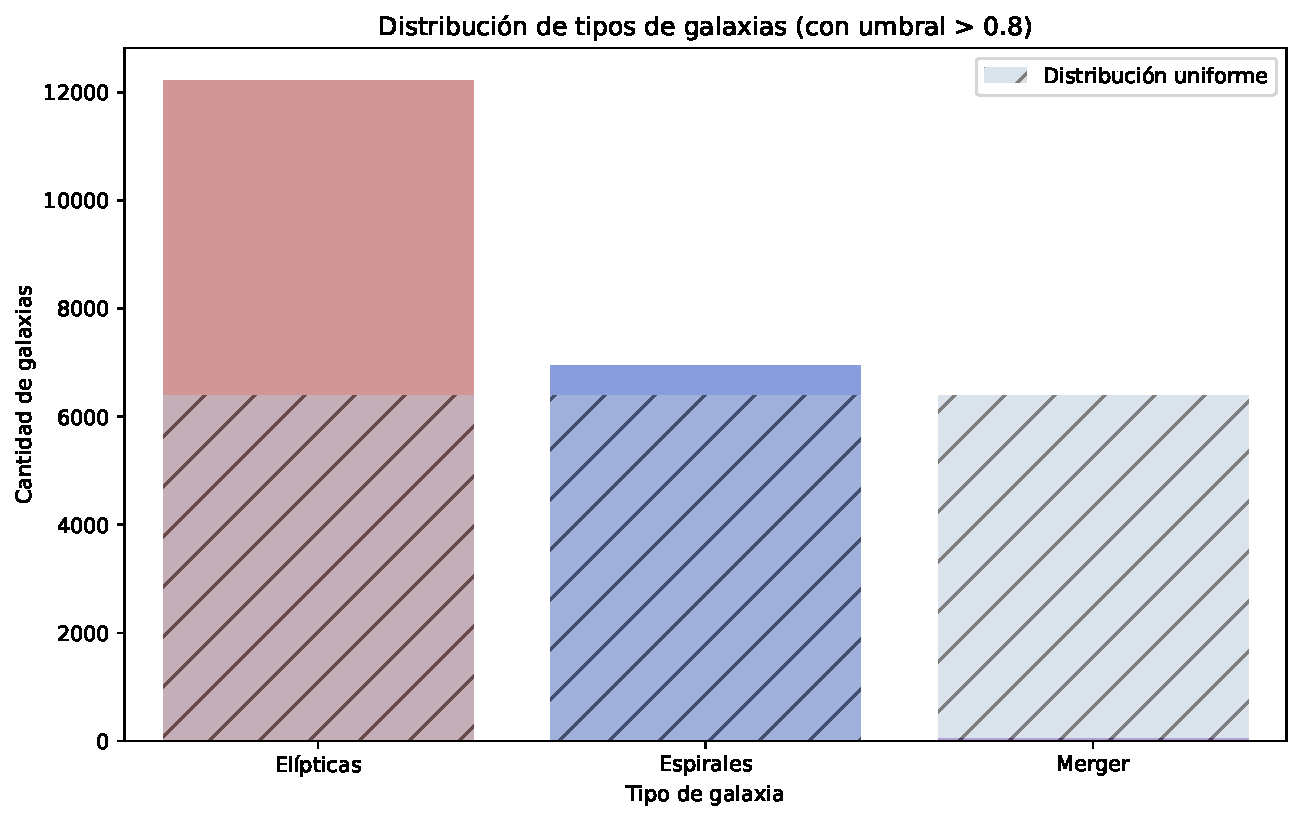
\includegraphics[width=\linewidth]{morfologia.pdf}
\caption{Histograma de la frecuencia de los tipos morfológicos de galaxias y superpuesto los valores esperados.}
\label{fig:morf}
\end{figure}
SDSS define un 3er tipo de magnitud que no se utilizó en este trabajo pero que dio pie a la definición del parámetro fracDeV dentro del catálogo; las \textit{Composite Model Magnitudes} o magnitudes módelo compuestas se definen a parit de una combinación lineal pesada de los perfiles de De Vaucoulers (galaxias elipticas) y : \[F_{\text{composite}} = fracDeV \,FdeV + (1 - fracDeV)\,Fexp\]. 
Por tanto $fraDeV$ es un parámetro en el cual se cuantiza que ``tanto'' se asemeja el pérfil de brillo respecto al pérfil de la ley de De Vaucoulers.\\
Este parámetro sirve como un primer \textit{approach} para conocer la componente principal de una galaxia, si $fracDeV \leq 0.2$ entonces el disco es prominente mientras que si $fracDeV \geq 0.8$ el bulbo es mas prominente. Lo cual sirve como un indicador de la forma de la galaxia.
Sin embargo al comparar ambos parámetros (\textit{ZooVotes} y \textit{FracDeV}) no se encuentra una correlación entre sí, lo que marca que no son intercambiables. 


\subsection{Magnitudes}
En este caso se trabajo con las magnitudes de las galaxias en 3 filtros $u$, $g$ y $r$ que son con los que cubren todo la región del óptico y que son los que se usan tipicamente para ver los colores de una galaxia. Hay especial enfasis en el filtro $r$ ya que es el que define SDSS como el filtro central y es el que se utiliza para definir los valores más fundamentales de una galaxia como el tamaño o su parámetro de concentración.

Con el punto de hacer un análisis preliminar y para ejemplificar el modelo de cuadrados mínimos explicado en la sección 1.1.3 se hizo un ajuste lineal para una submuestra del $10\%$ de la muestra total (no de toda la muestra por costo computacional) y de las submuestras de las galaxias elípiticas y espirales, con lo que obtuvimos los gráficos que se muestran en la figura \ref{fig:lineal}

\begin{figure*}[ht]
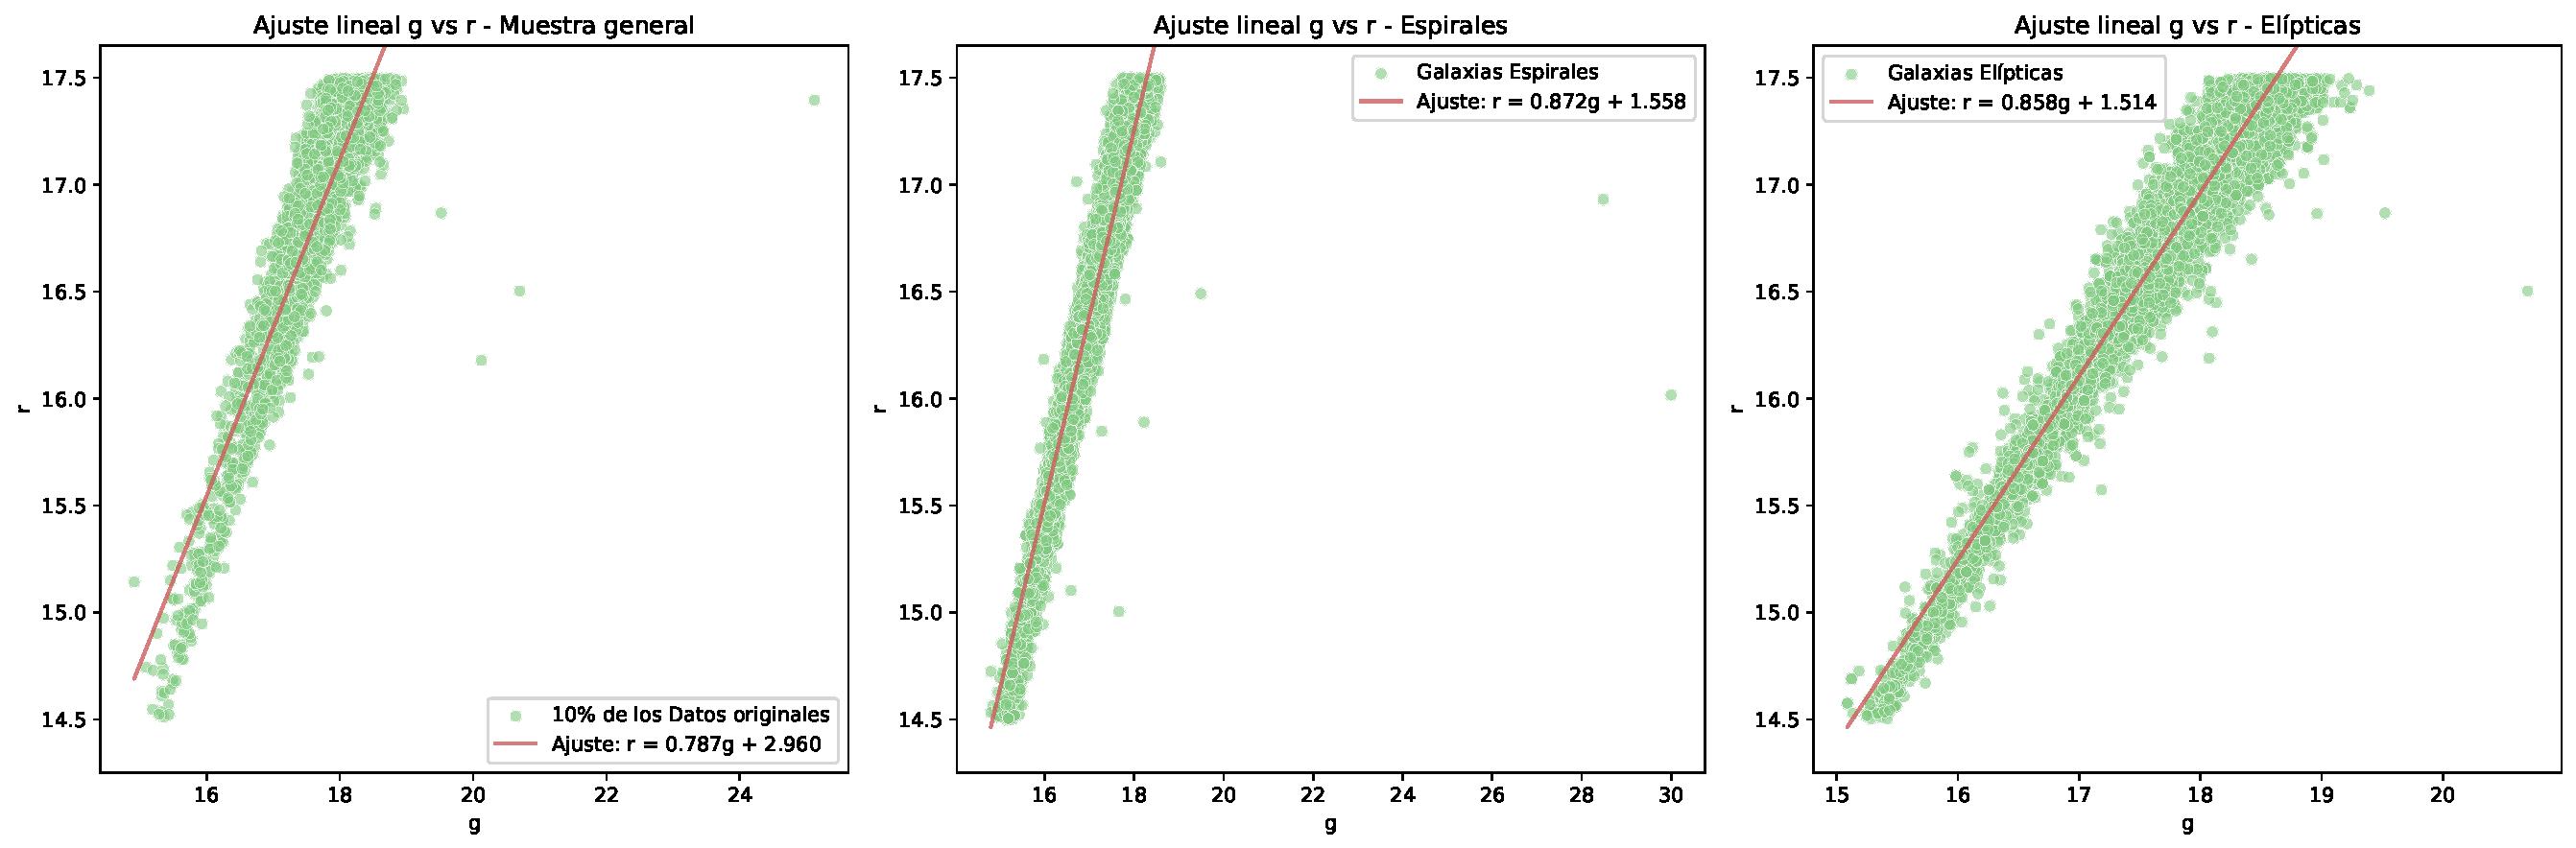
\includegraphics[width=\linewidth]{ajustes_lineales_comparacion.pdf}
\caption{Ajuste lineal $g$ vs $r$ para 3 submuestras distintas.}
\label{fig:lineal}
\end{figure*}

\subsubsection{Magnitud Absoluta}
Como las galaxias son objetos a unas distancias muy grandes ya los efectos de la relatividad general se aplican al momento de calcular el módulo de la distancia, pues el redshift enrojece tanto a la galaxia que afecta la medida de distancia. Existe un desarrollo al partir del cual podemos medir una \textit{distancia luminosa} la cual nos permite calcular el módulo de la distancia, en este trabajo se aplico una aproximación a la misma tomando que la magnitud absoluta esta dada por:
\begin{equation}
M_r= r - 25 -5log\left(\frac{c·z}{H_0}\right)
\end{equation}
donde $c=30000km s^{-1}$ es la velocidad de la luz, $H_0=75 km s^{-1}Mpc^{-1}$ es la constante de Hubble y $z$ es el valor del redshift de cada galaxia.
Al hacer esto obtenemos la figura \ref{fig:mabs} donde se ve que los puntos parecieran estar delimitados por una curva logarítmica (ver figura \ref{fig:mabs_log}) lo que se debe a la extinción por $z$, ya que a mayor redshift mayor el enrojecimiento y menor el flujo que recibimos del objeto, por lo que las galaxias mas debiles se vuelven ``invisibles''. 
\begin{figure}[t]
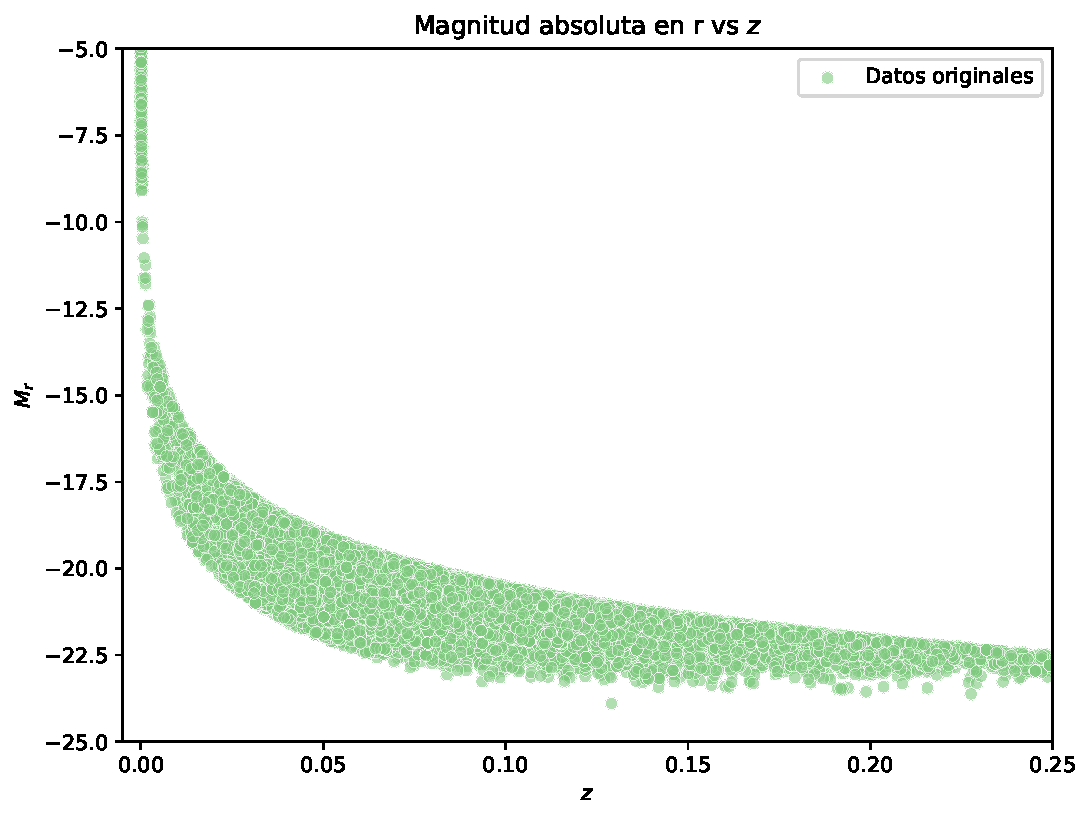
\includegraphics[width=\linewidth]{mabs.pdf}
\caption{Magnitud absoluta en el filtro $r$ vs corrimiento al rojo $z$.}
\label{fig:mabs}
\end{figure}

\begin{figure}[t]
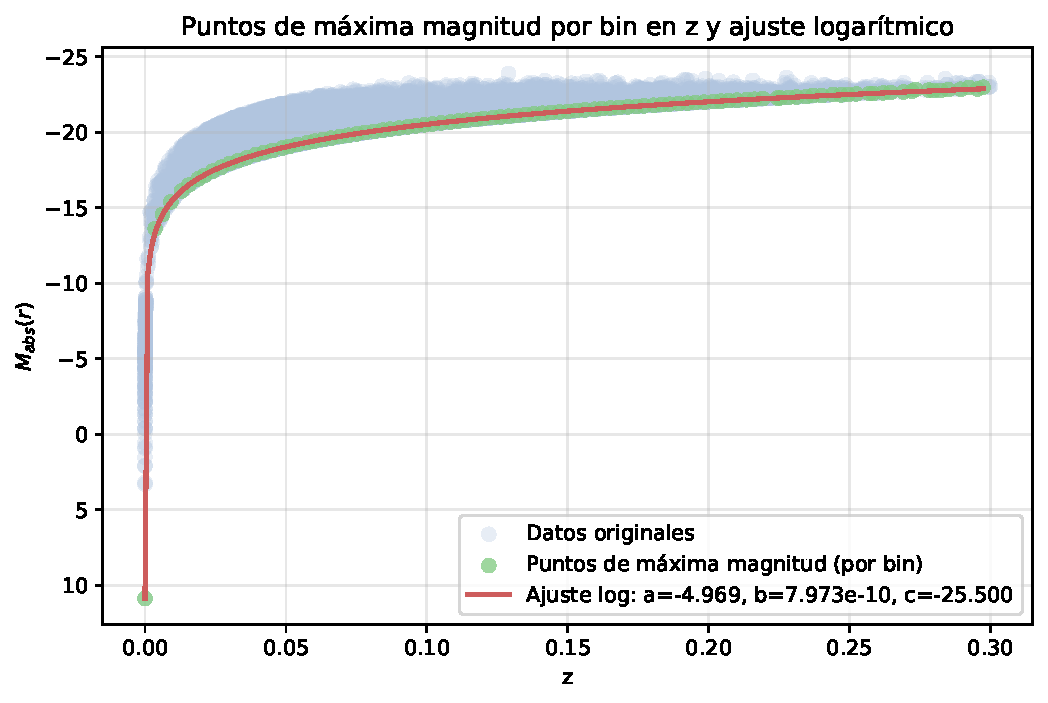
\includegraphics[width=\linewidth]{mabs_vs_z_ajuste_log_max.pdf}
\caption{Magnitud absoluta en el filtro $r$ vs corrimiento al rojo $z$. Superpuesto el ajuste para la envolvente de los puntos.}
\label{fig:mabs_log}
\end{figure}



\subsection{Análisis de color}
Gracias a \citet{2004Bimodalidad} sabemos que todas las muestras de galaxias presentan una distribución bimodal en la distribución del color a la cual le podemos ajustar una doble gaussiana, que nos permite separar las galaxias en las que son color rojo (es decir que tienen $u-r$ alto) y las que son color azul que tienen un $u-r$ bajo. 
En la figura \ref{fig:ur}
\begin{figure}[t]
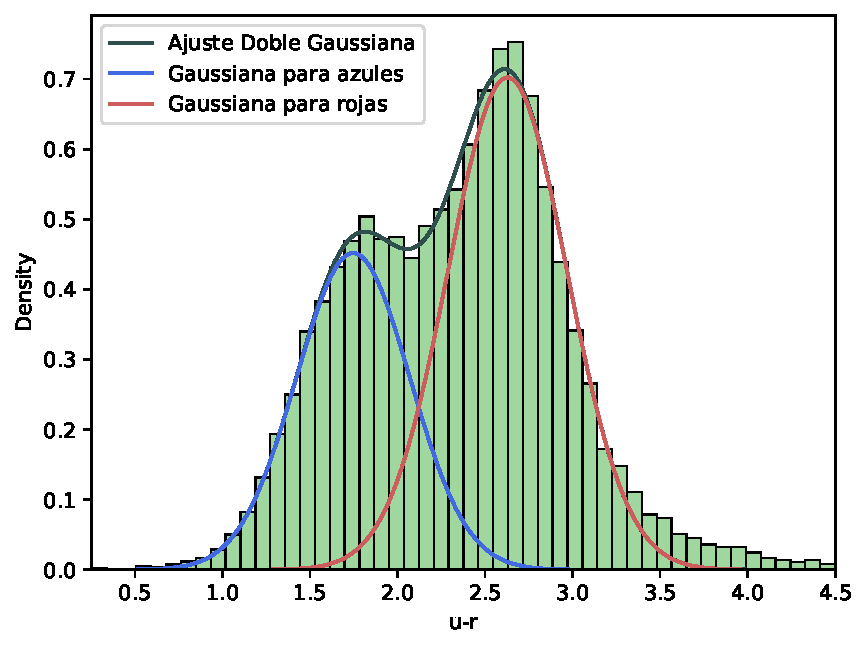
\includegraphics[width=\linewidth]{ur.pdf}
\caption{Histograma del color $u-r$ de las galaxias seleccionadas. Por encima ajuste de la doble gaussiana y cada gaussiana por separado.}
\label{fig:ur}
\end{figure}
Una vez que obtenemos estos valores usamos el test de chi-cuadrado con las funciones de la libreria de \textit{SciPy} \citep{SciPy} para comprobar si este modelo es aceptable

Esto mismo lo repetimos para los distintos colores que podemos trabajar con la galaxia. Se eligió  el color $u-r$ para comenzar por que utiliza los filtros que estan mas alejados entre si y que por lo tanto presenta la mayor diferencia entre los picos, esto se puede ver claramente en la figura \ref{fig:colores}.

\begin{figure}[t]
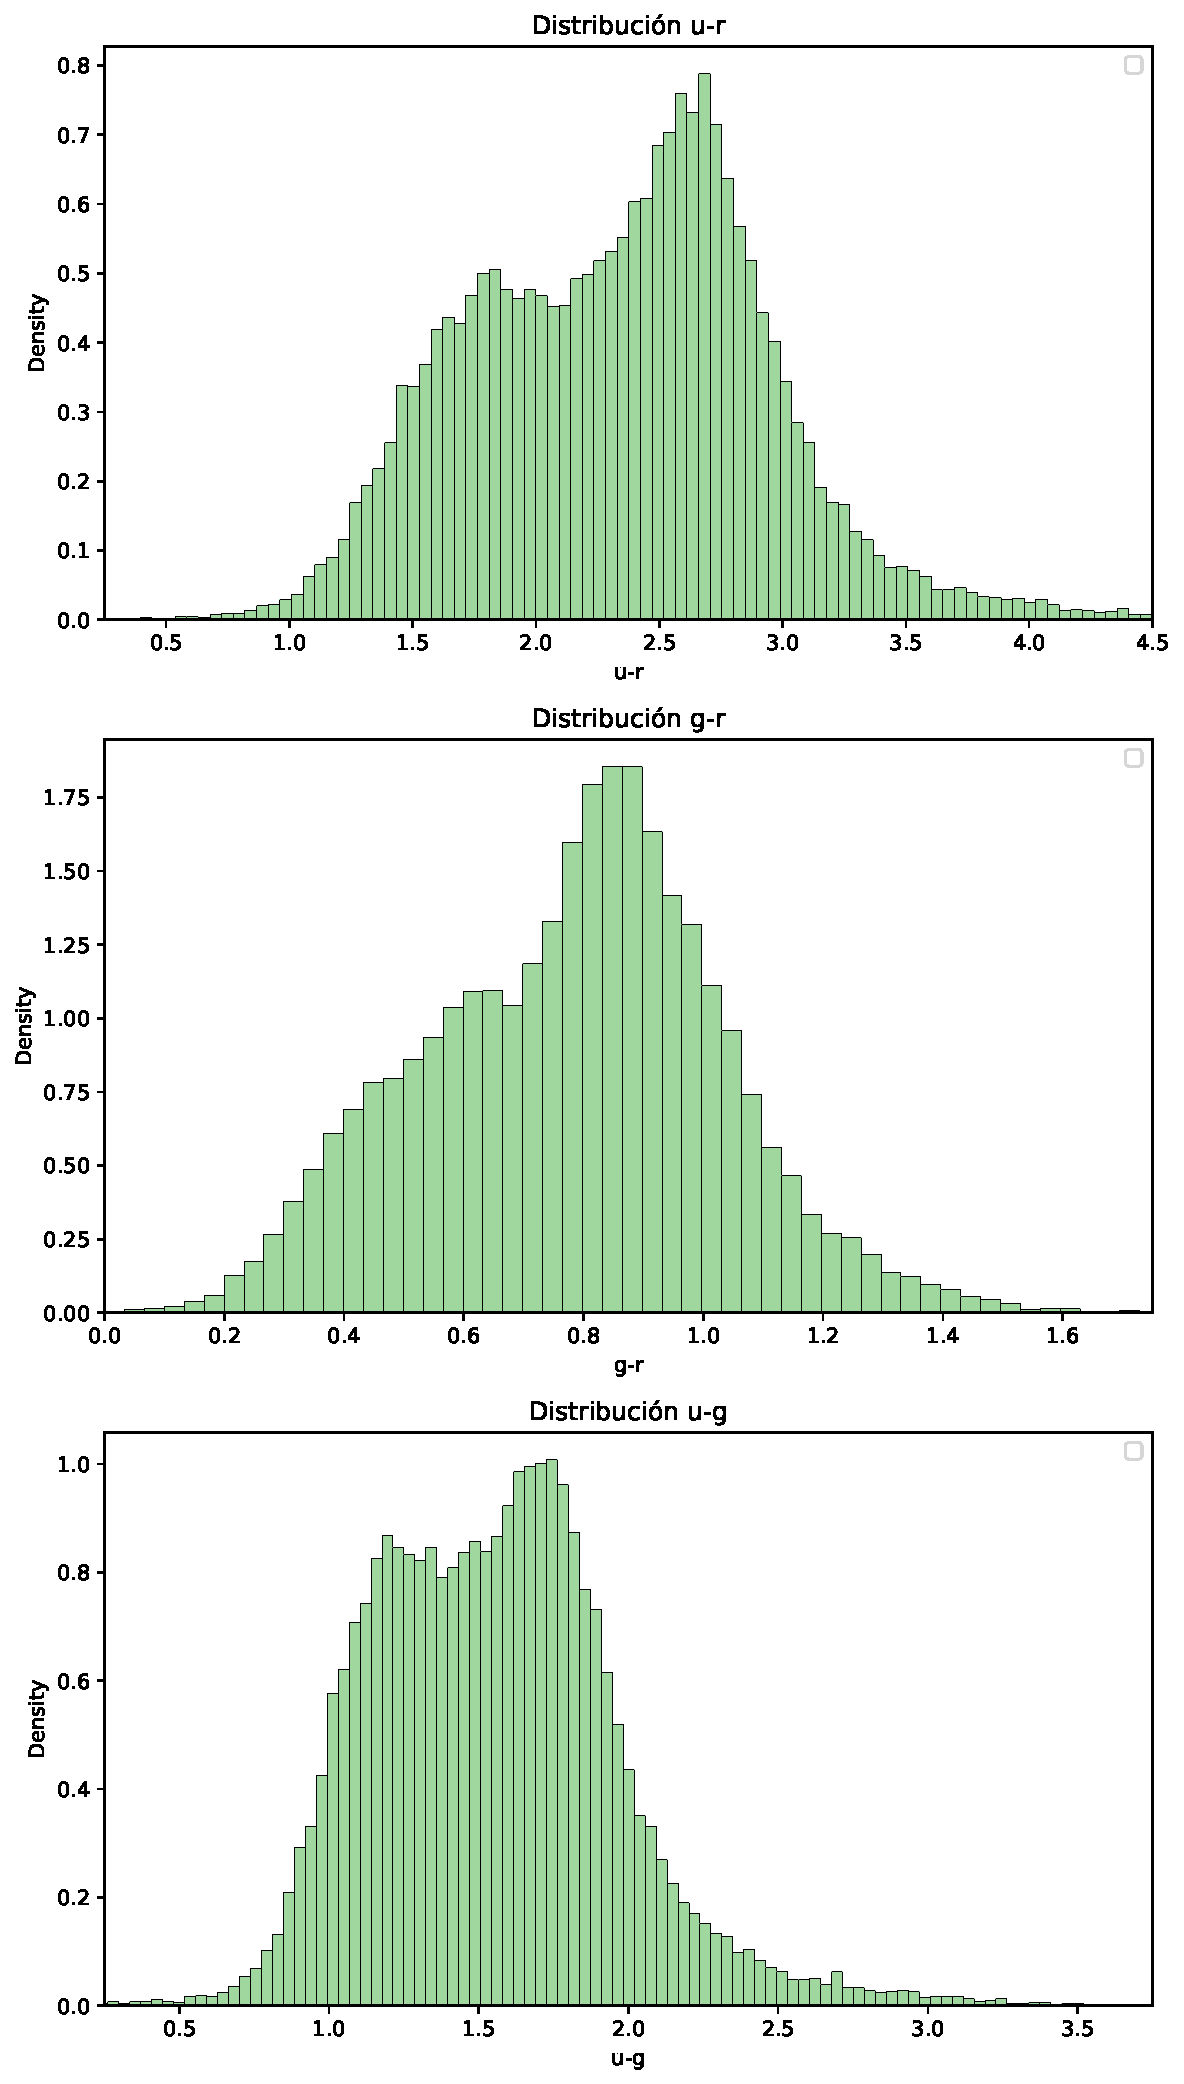
\includegraphics[width=\linewidth]{rojas_azules_vertical.pdf}
\caption{Histograma del color $u-r$,$g-r$ y $u-g$  de las galaxias seleccionadas.}
\label{fig:colores}
\end{figure}

Ahora se realizo este mismo análisis pero separando según la moroflogía y se observa en la figura \ref{fig:color_forma} que primeramente las distribuciones de cada tipo de galaxia por separado perdió la bimodalidad que se marcaba en la muestra total, pero ademas en todos los casos las espirales son sistematicamente mas azules que las elípticas. 
Para verificar si su distribución es semejante entre si se aplicó el test de chi-cuadrado y en todos los casos se obtuvo que las formas no son las mismas. Esto nos intuye que hay una relación entre color y la morfología de las galaxias.

\begin{figure}[t]
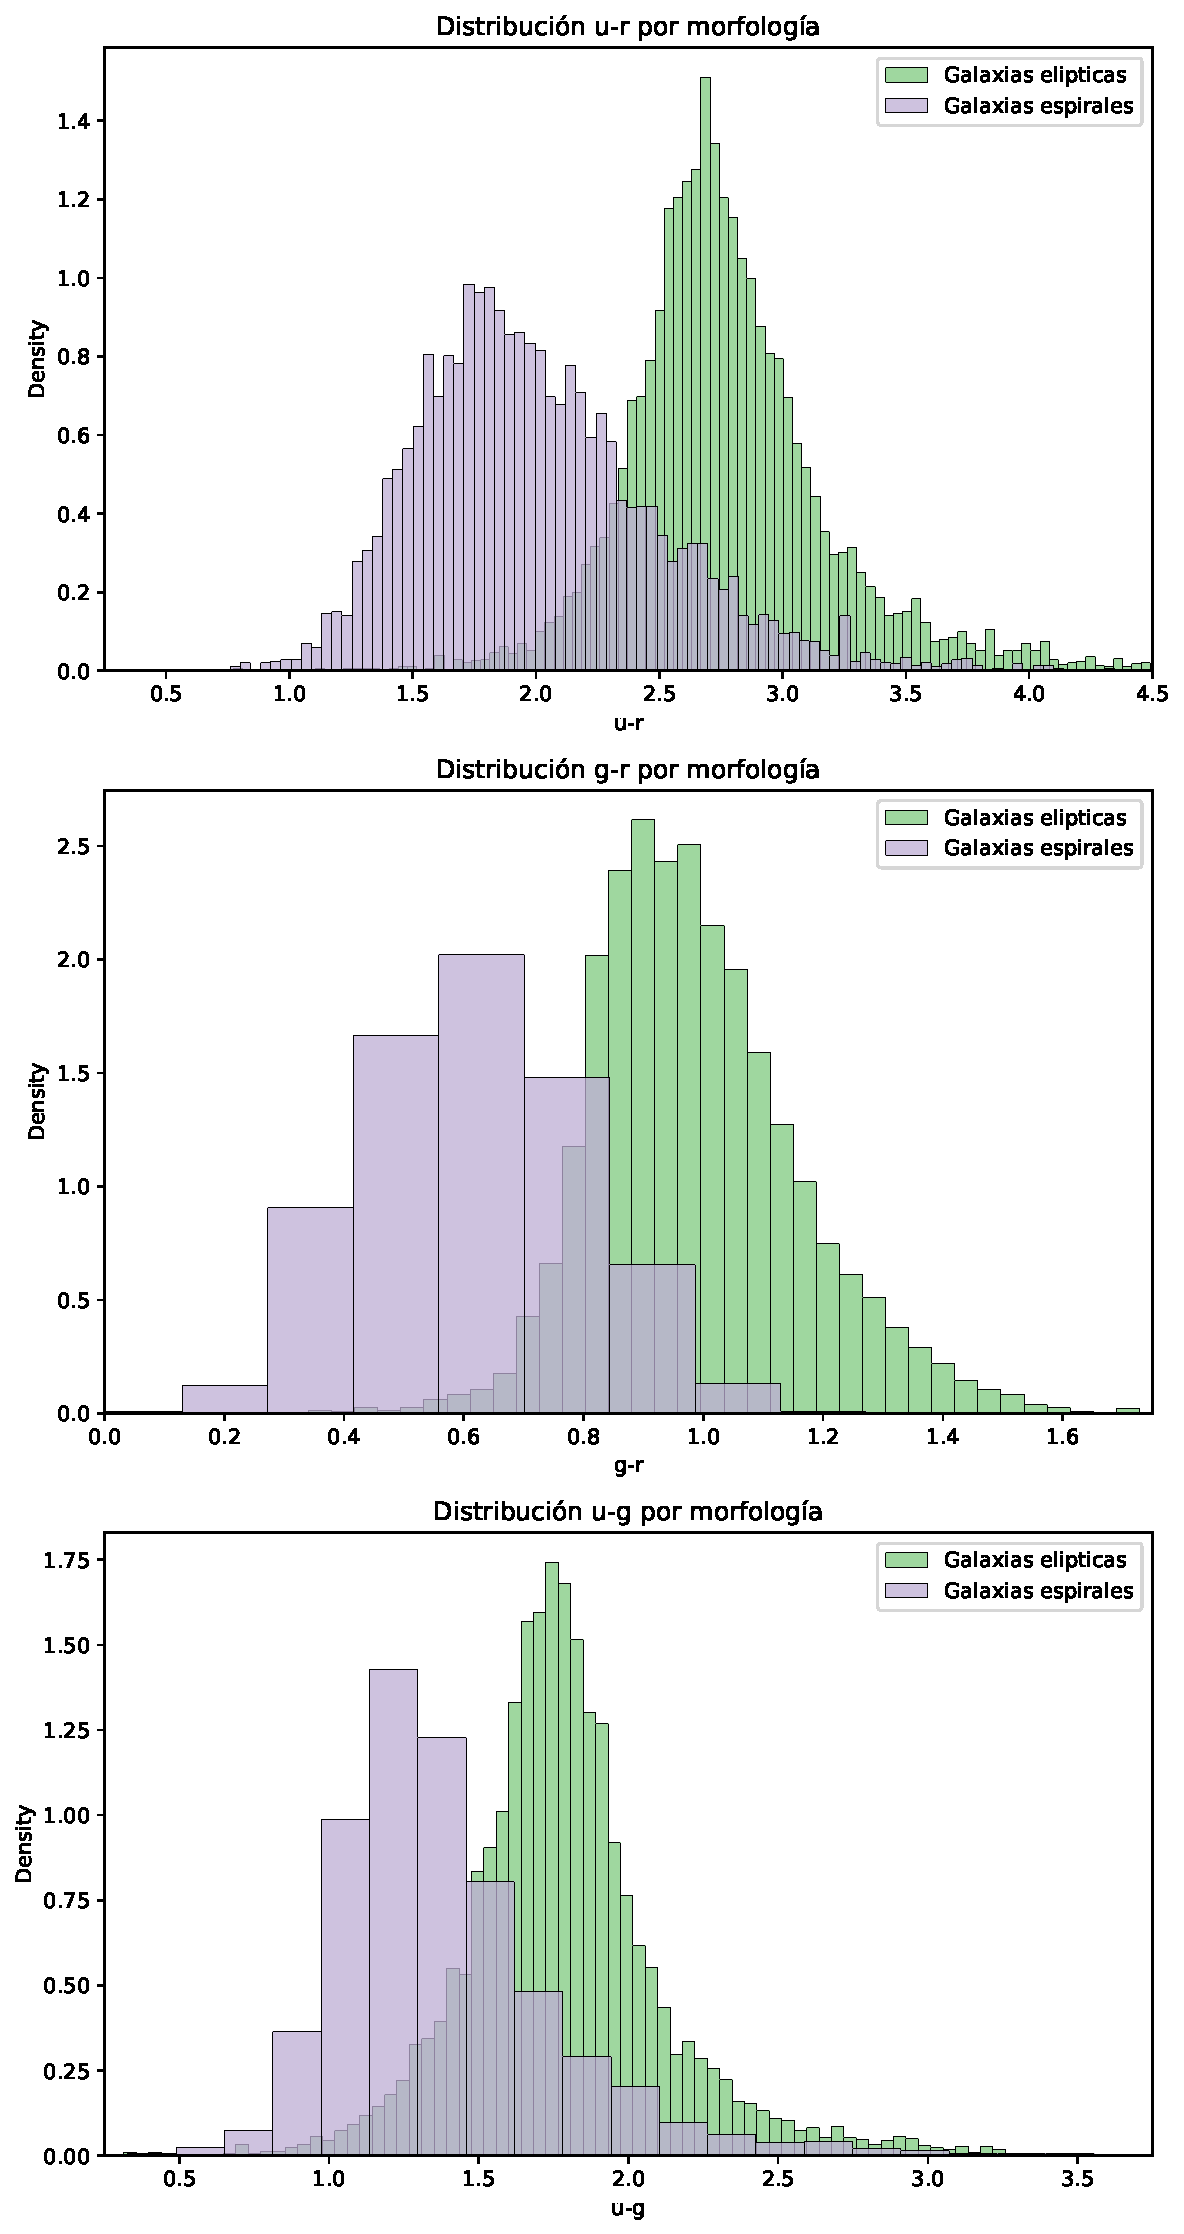
\includegraphics[width=\linewidth]{colores_morfologia_vertical.pdf}
\caption{Histograma del color $u-r$,$g-r$ y $u-g$  de las galaxias espirales y elípticas.}
\label{fig:color_forma}
\end{figure}



\section{Conclusiones}
Se nota como el analisis estadistico y el modelado de datos es esencial para la astronomía. En este trabajo se mostró como la información que se puede extraer de las distribuciones de gran cantidades de galaxias nos permitió ver sus características, como que las galaxias elípticas son más rojas que las espirales o que a mayor redshift se pierden aquellas galaxias de menor brillo. 

\bibliographystyle{plainnat}
\bibliography{bibliografia}

\end{document}